% arara: pdflatex
\documentclass{report}
\usepackage{graphicx}
\usepackage{xcolor}
\usepackage{forest}
\usepackage{amsmath}
\renewcommand{\chaptername}{Section}
\begin{document}
\begin{titlepage}
\begin{center}
	\vspace*{1cm}

	\Huge
	\textbf{Course Project}

	\vspace{0.5cm}
	\LARGE
	Second Deliverable: The Parser	

	\vspace{1.5cm}

	\textbf{Quin'darius Lyles-Woods}
	\Large
	qlyleswo@students.kennesaw.edu

	\vfill
	\LARGE
	Concepts of Programming Languages	\\
	Professor Jose Garrido			\\
	Section W01 				\\
	4308
	\vspace{0.8cm}

	
\includegraphics[width=\textwidth]{kennesawlogo}

	\vspace{0.8cm}

	\Large
	Bachelors of Computer Science\\
	Kennesaw State University\\
	1100 South Marietta Pkwy SE\\
	Marietta, GA 30060\\
	\today	

	\vspace{1cm}

\end{center}
\end{titlepage}


\section*{Task}
The development of a python program to manage course information for the user. 

\vspace{0.5cm}

\subsection*{Assignment Goals}
\begin{itemize}

	\item Define a class for a Course Object 
	\item Allow the user to add a new course object  
	\item Allow the user to change the course object  
	\item List all the courses that have been added to the list
\end{itemize}

\subsection*{Source Code}
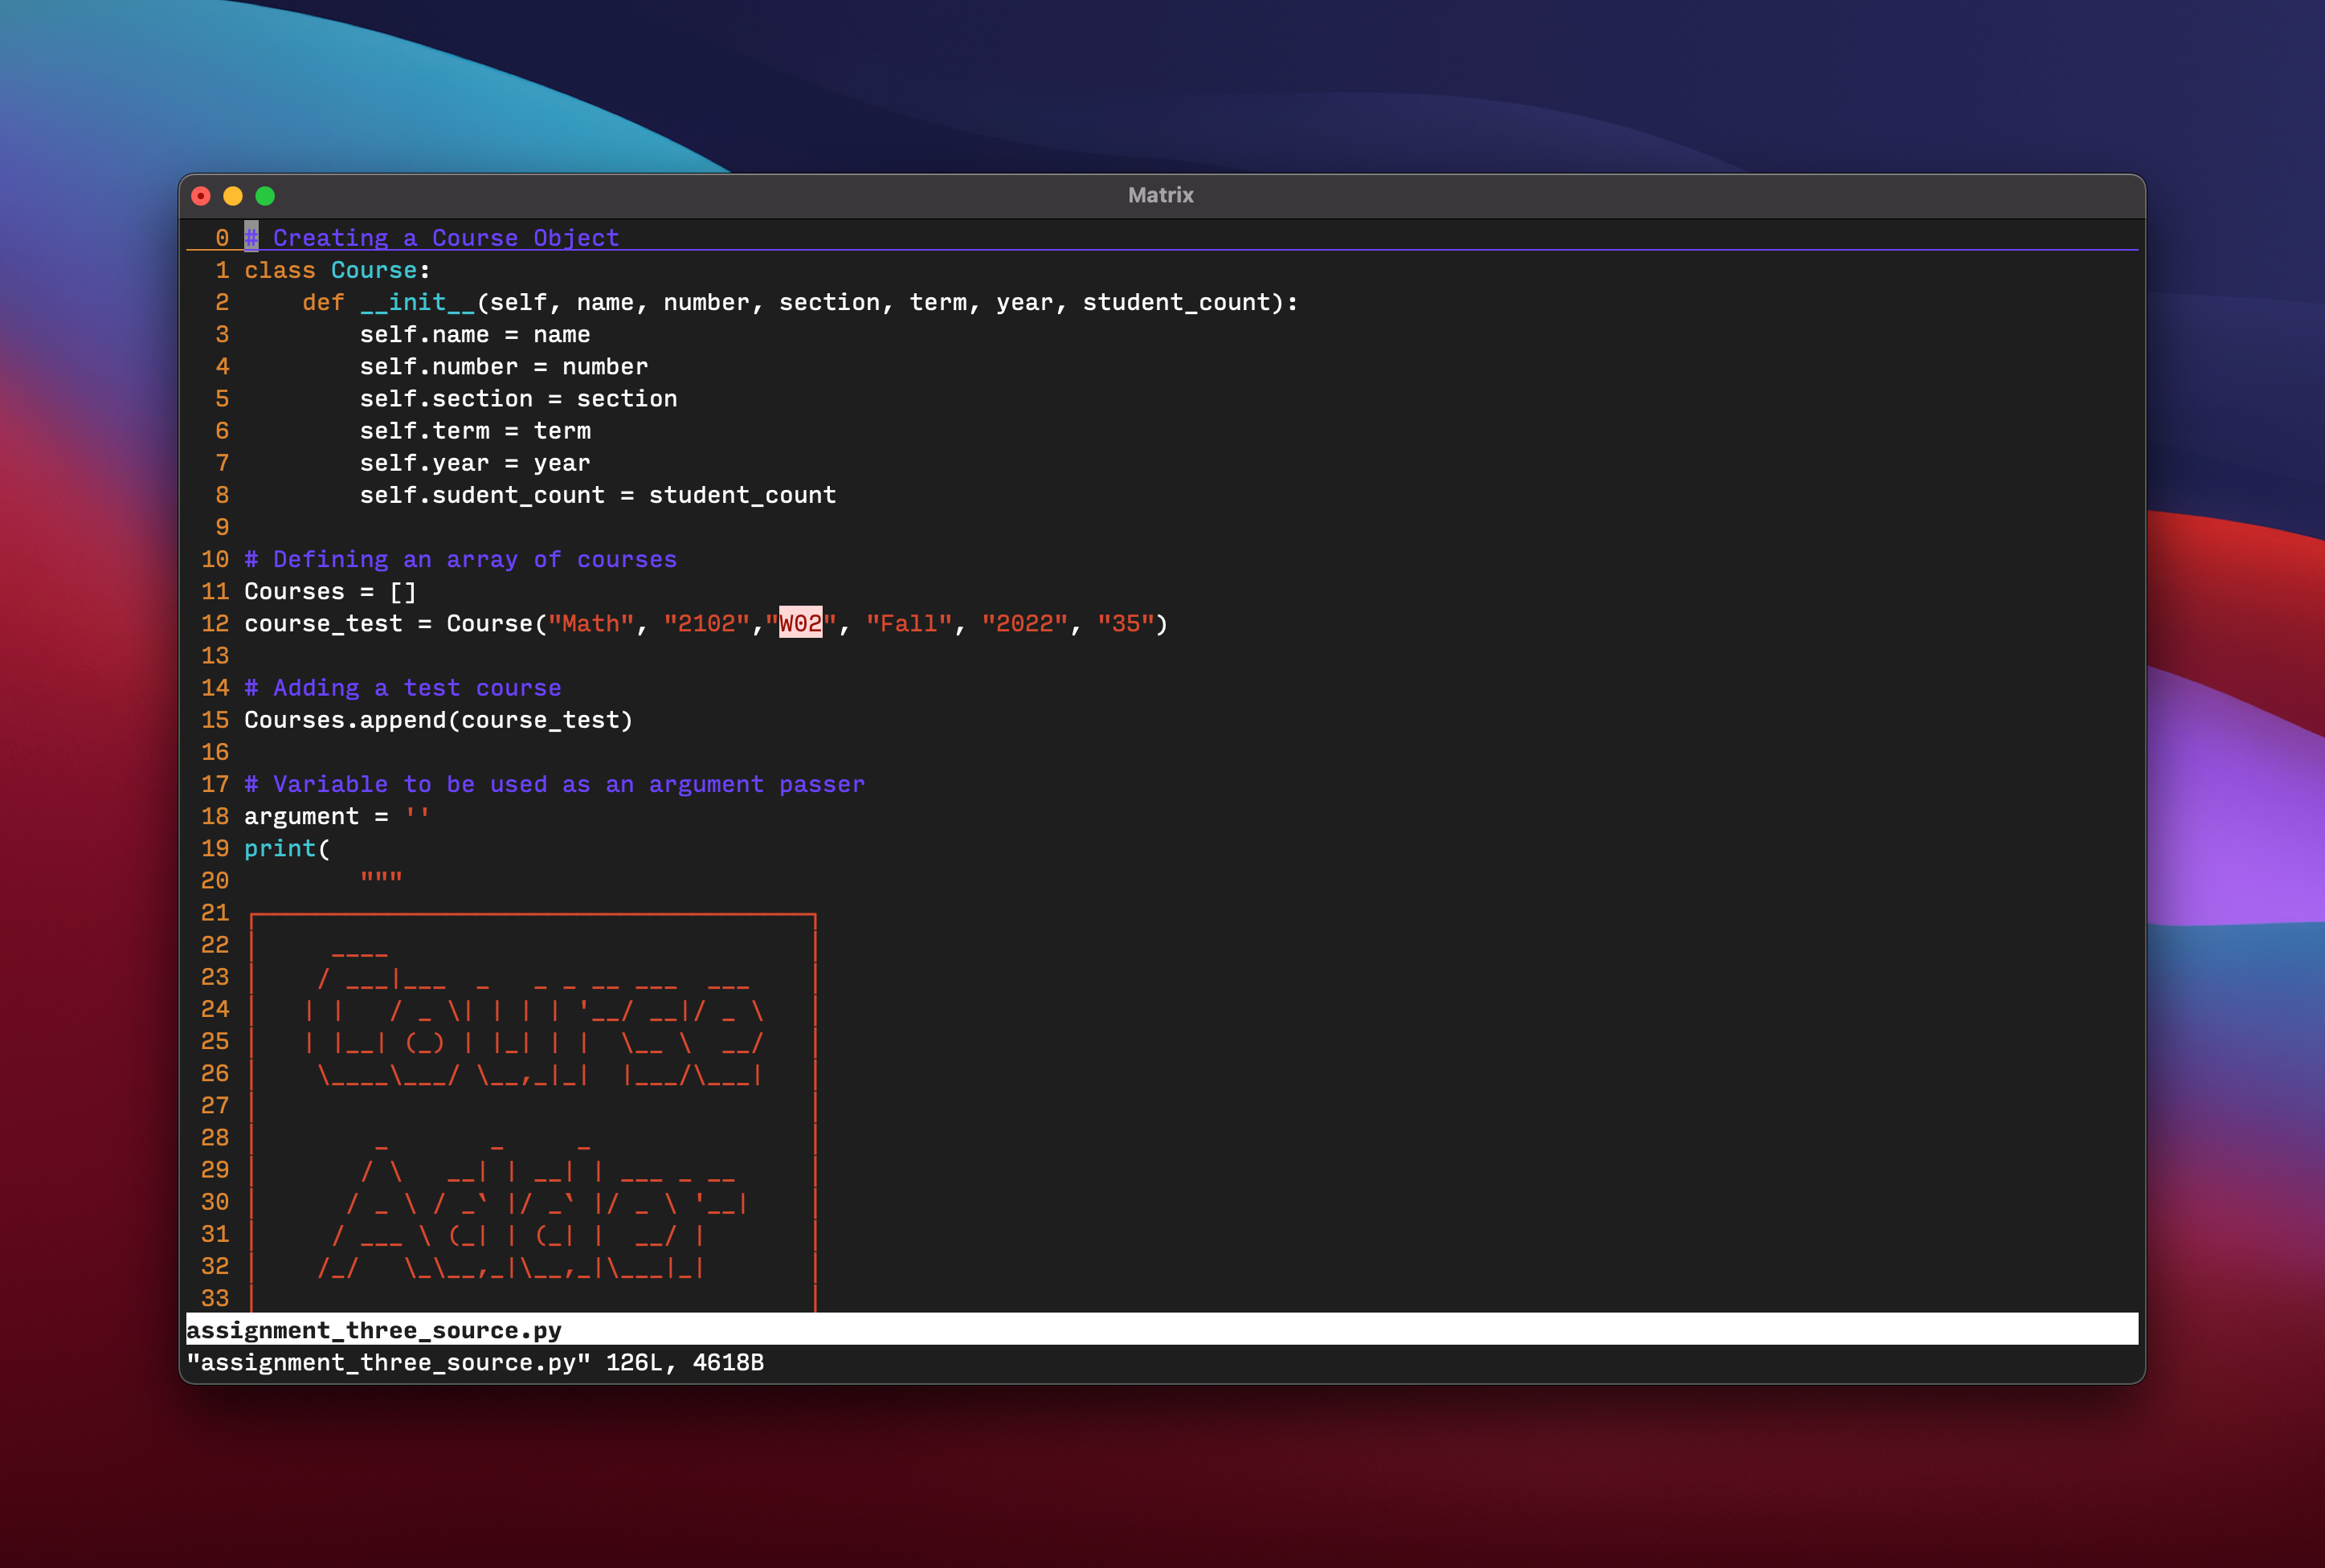
\includegraphics[width = \textwidth]{source}
\subsection*{Run Output}
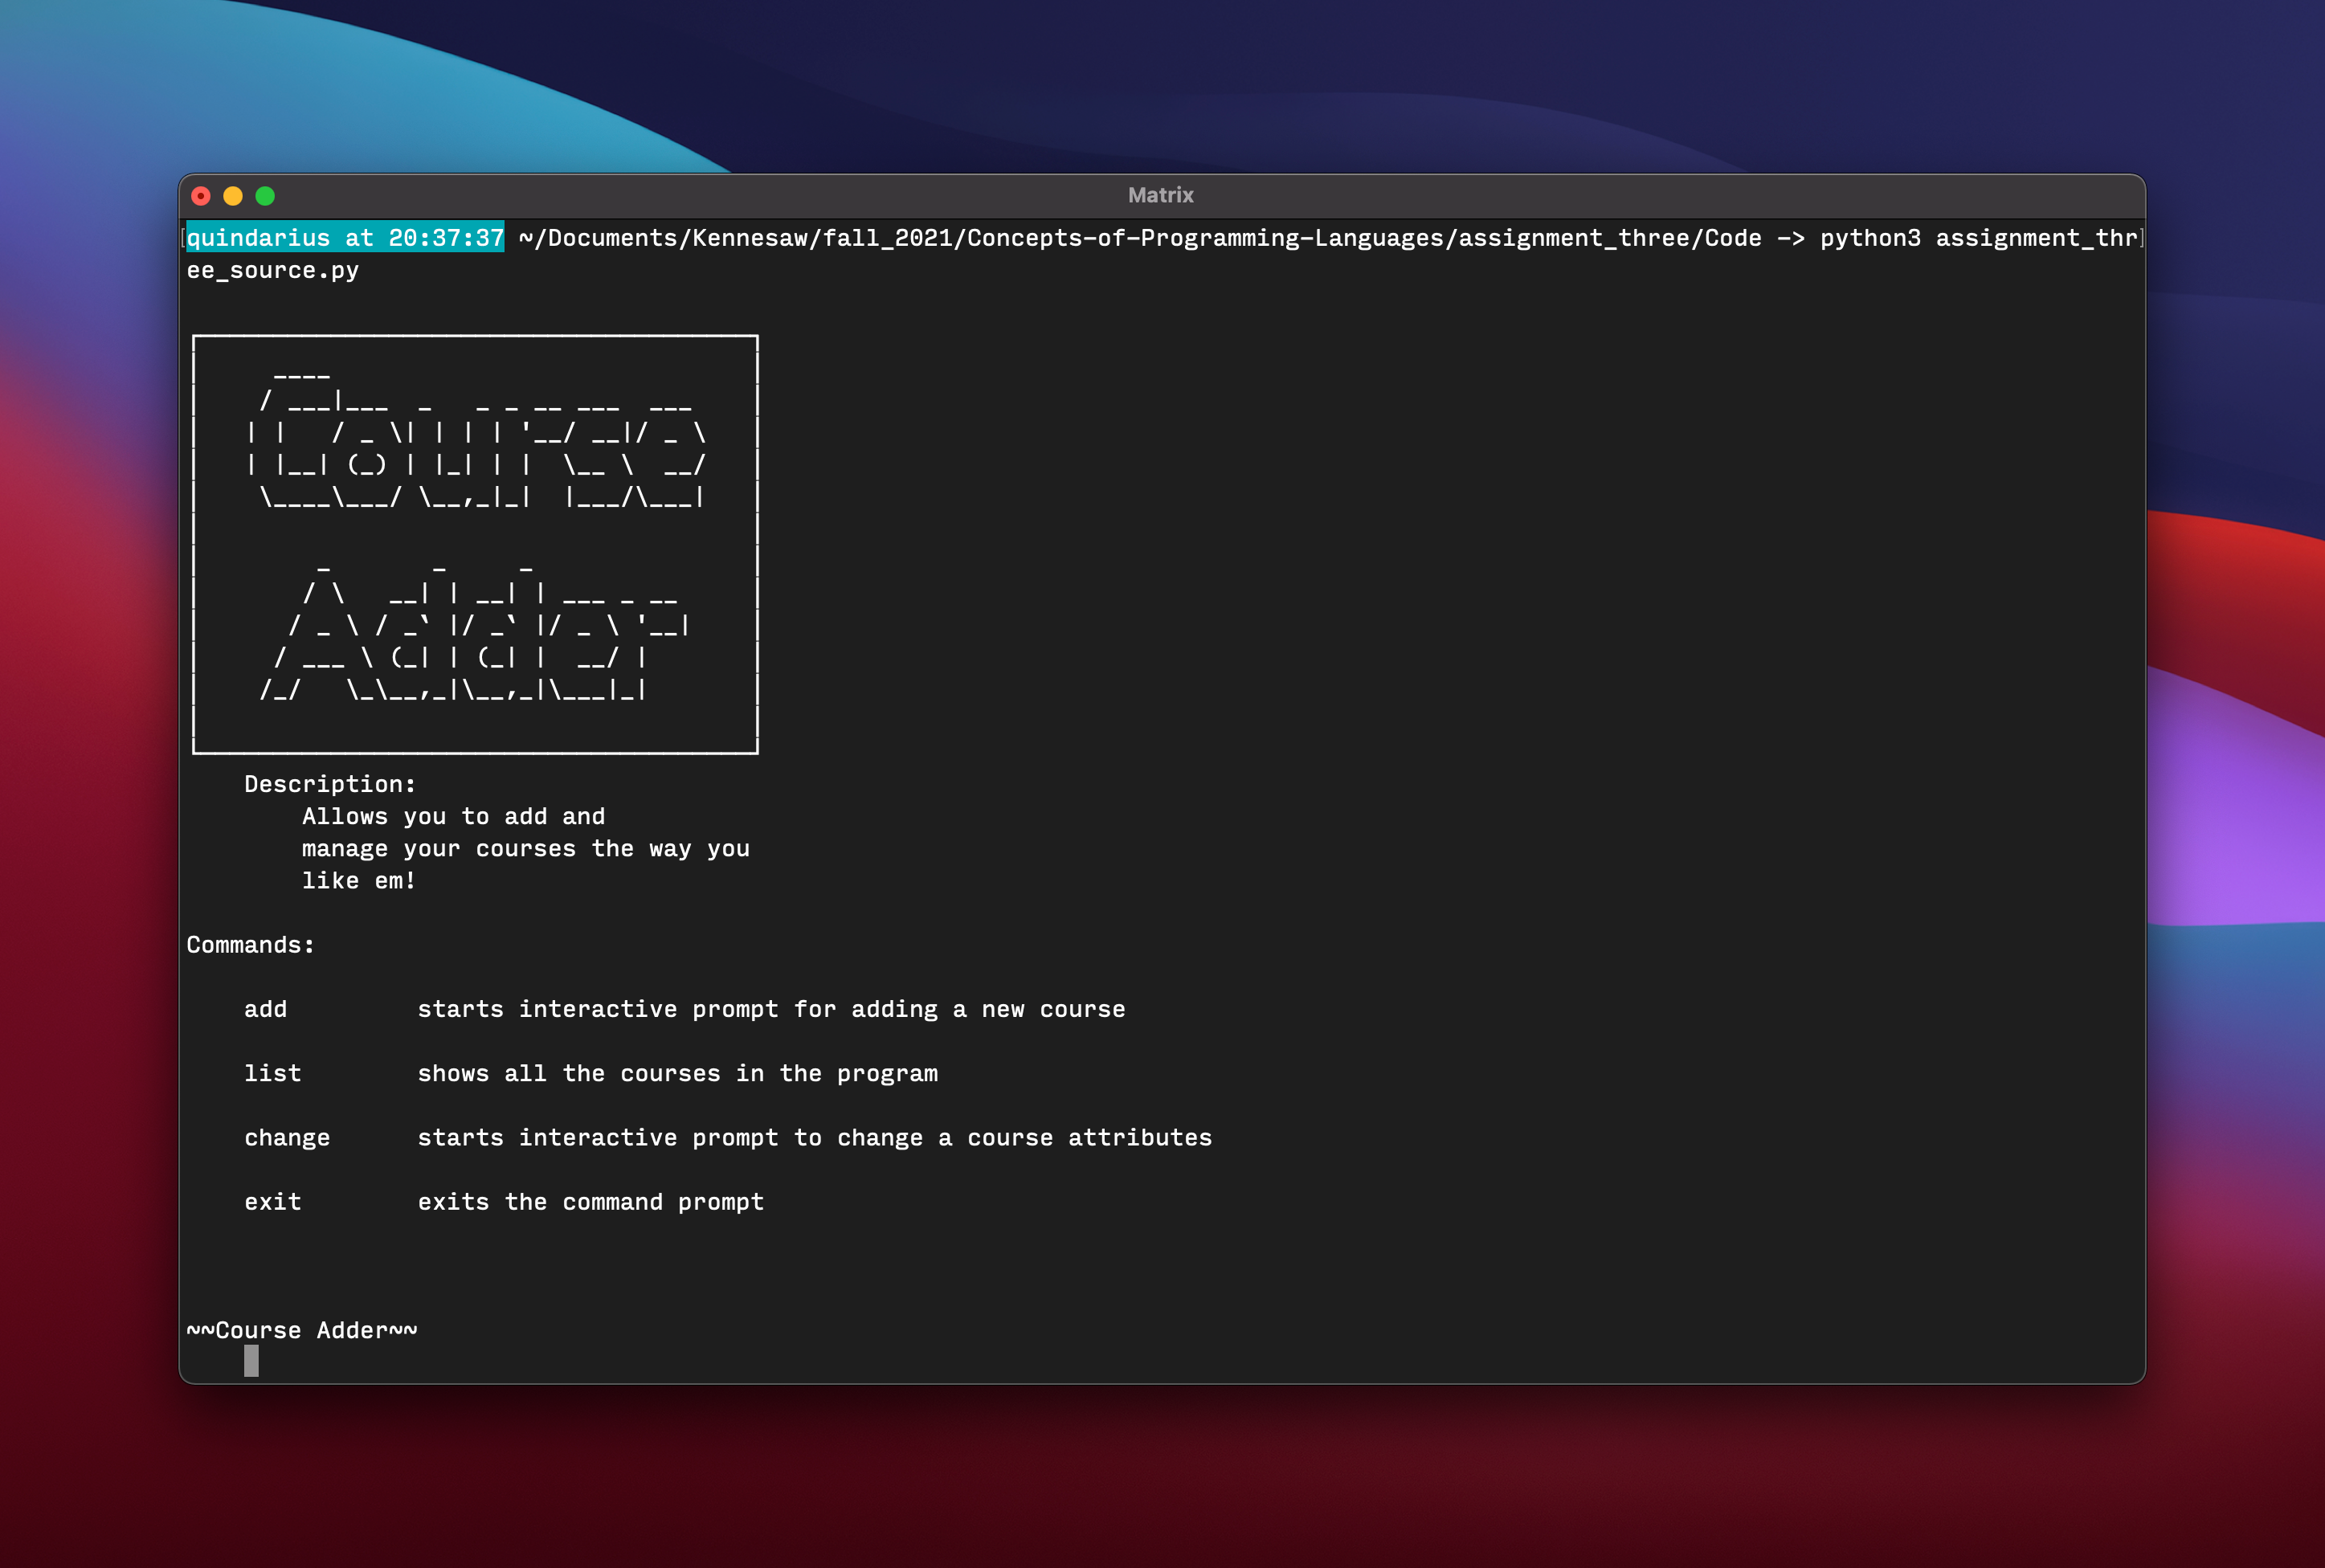
\includegraphics[width = \textwidth]{run}
\subsection*{Add Output}
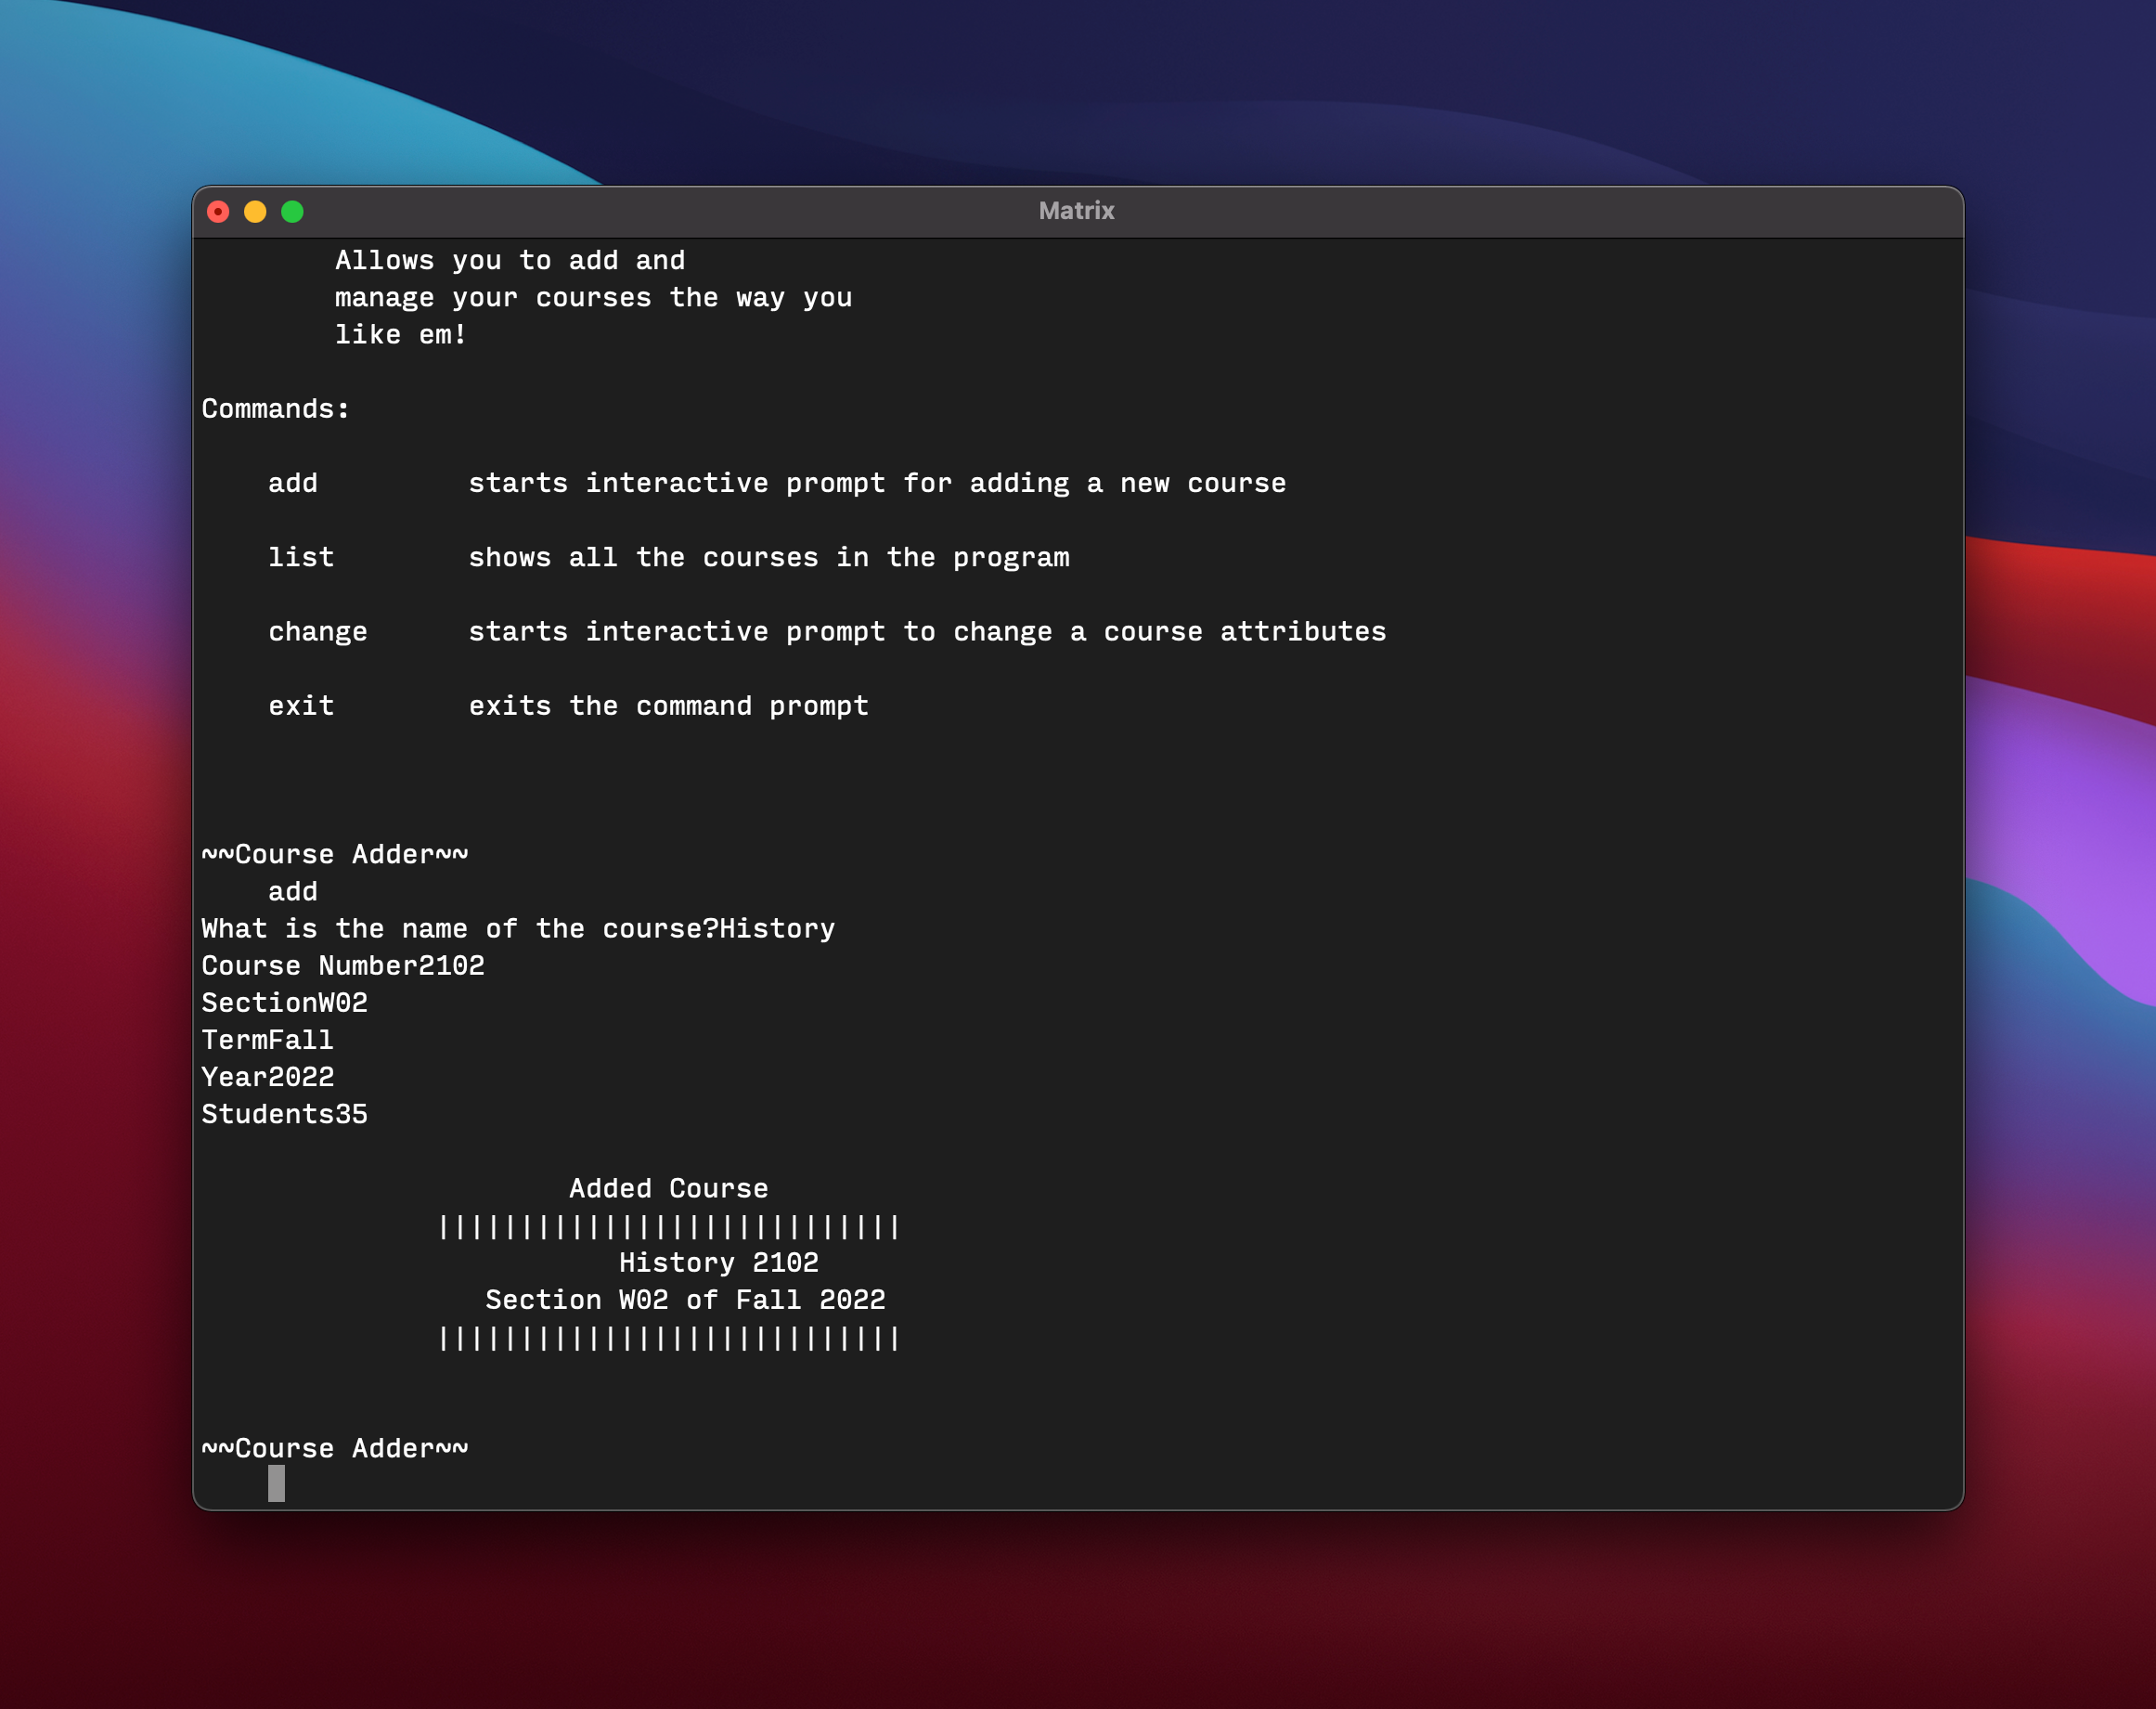
\includegraphics[width = \textwidth]{add}
\subsection*{List Output}
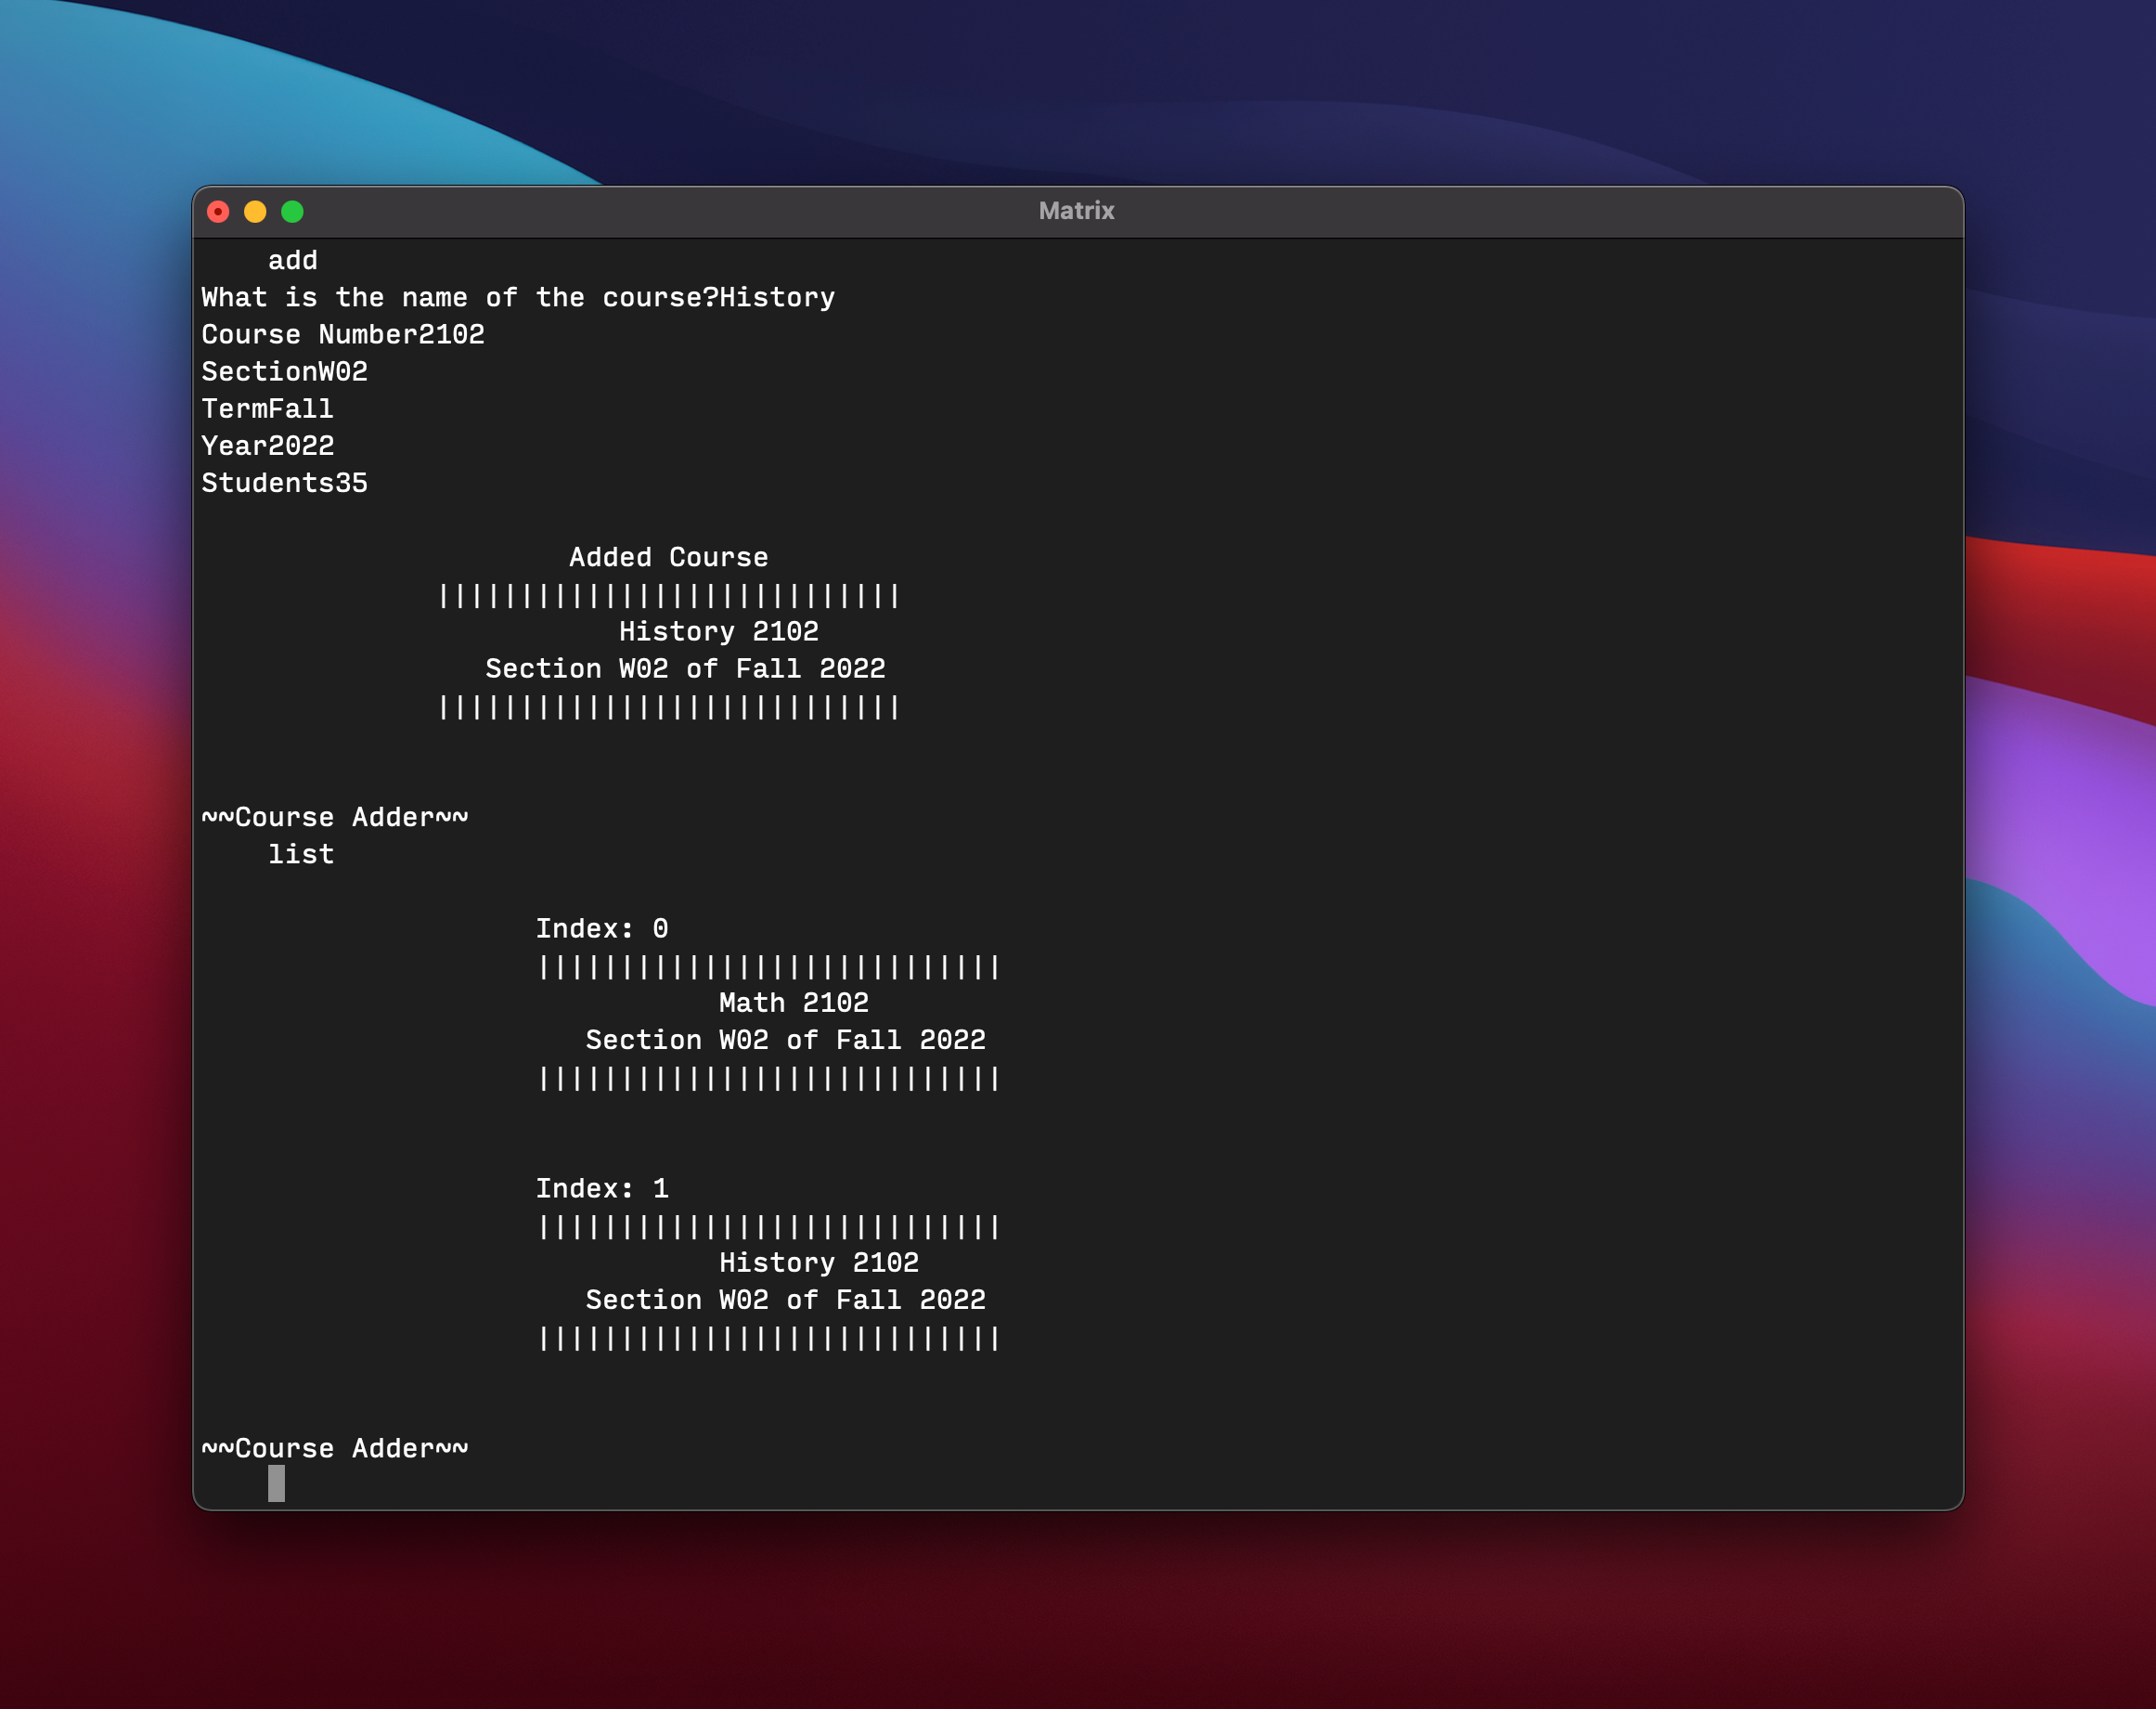
\includegraphics[width = \textwidth]{list}
\subsection*{Change Output}
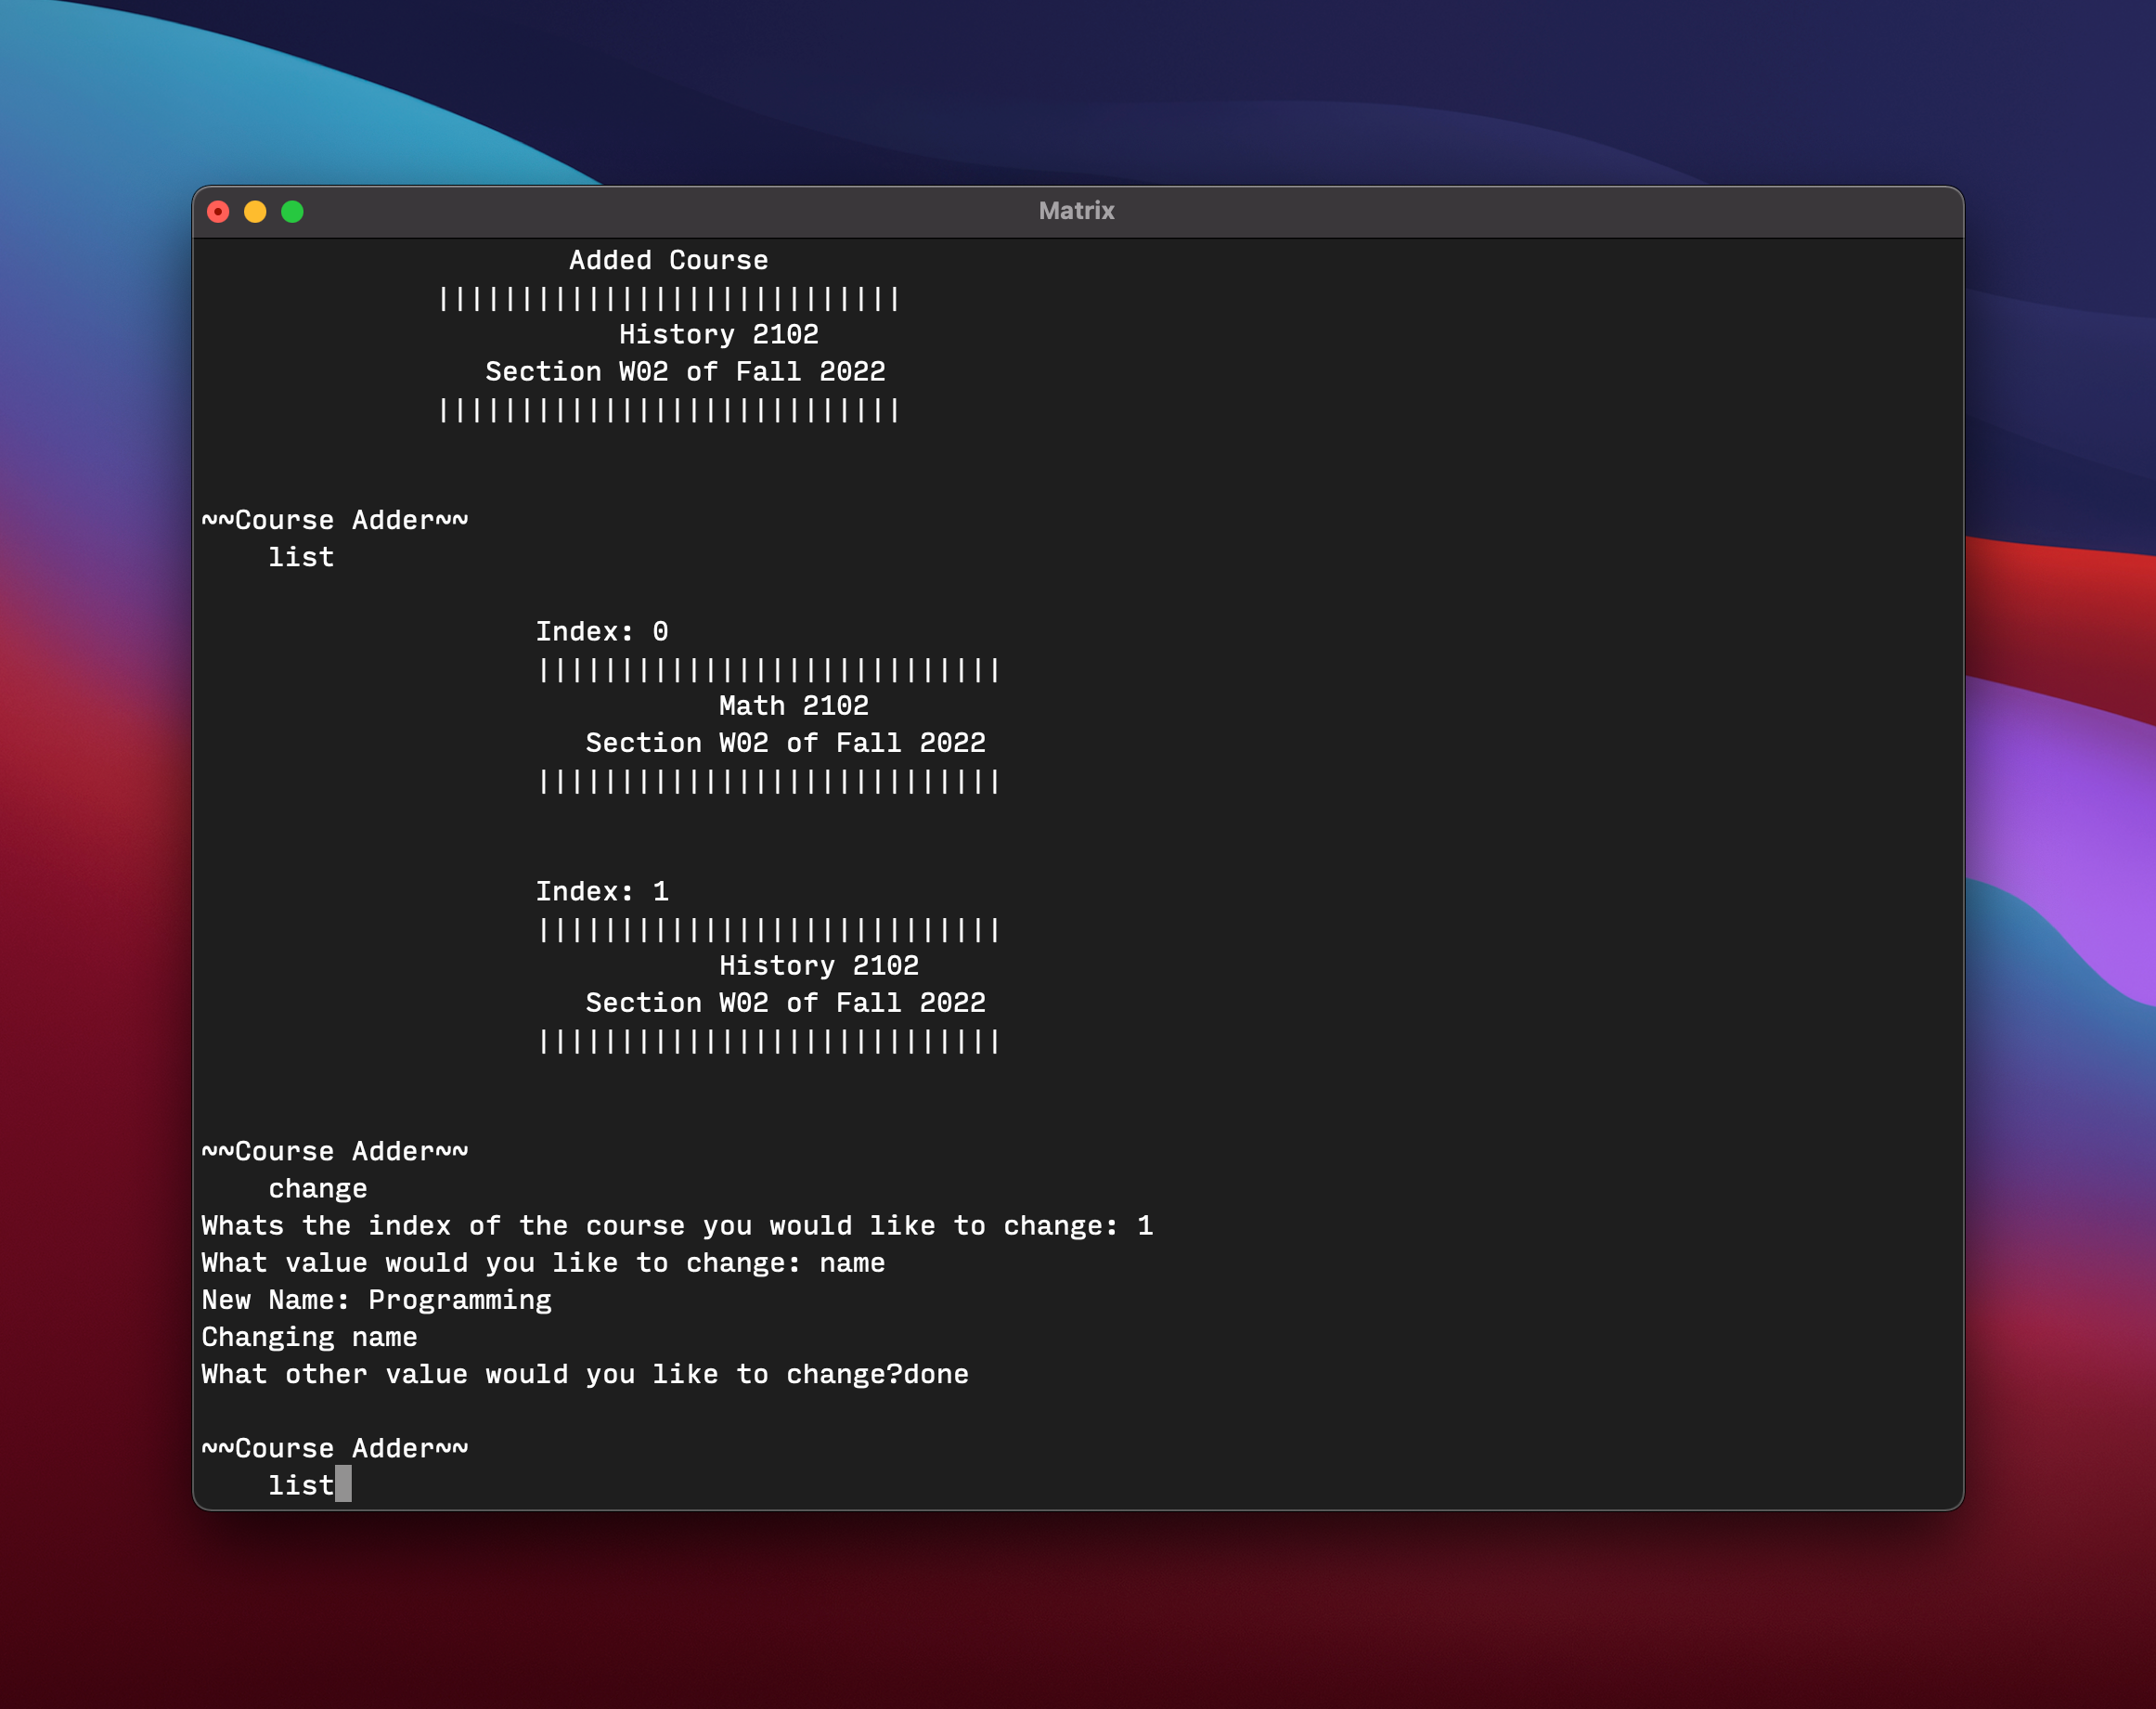
\includegraphics[width = \textwidth]{change}
\subsection*{List After Change Output}
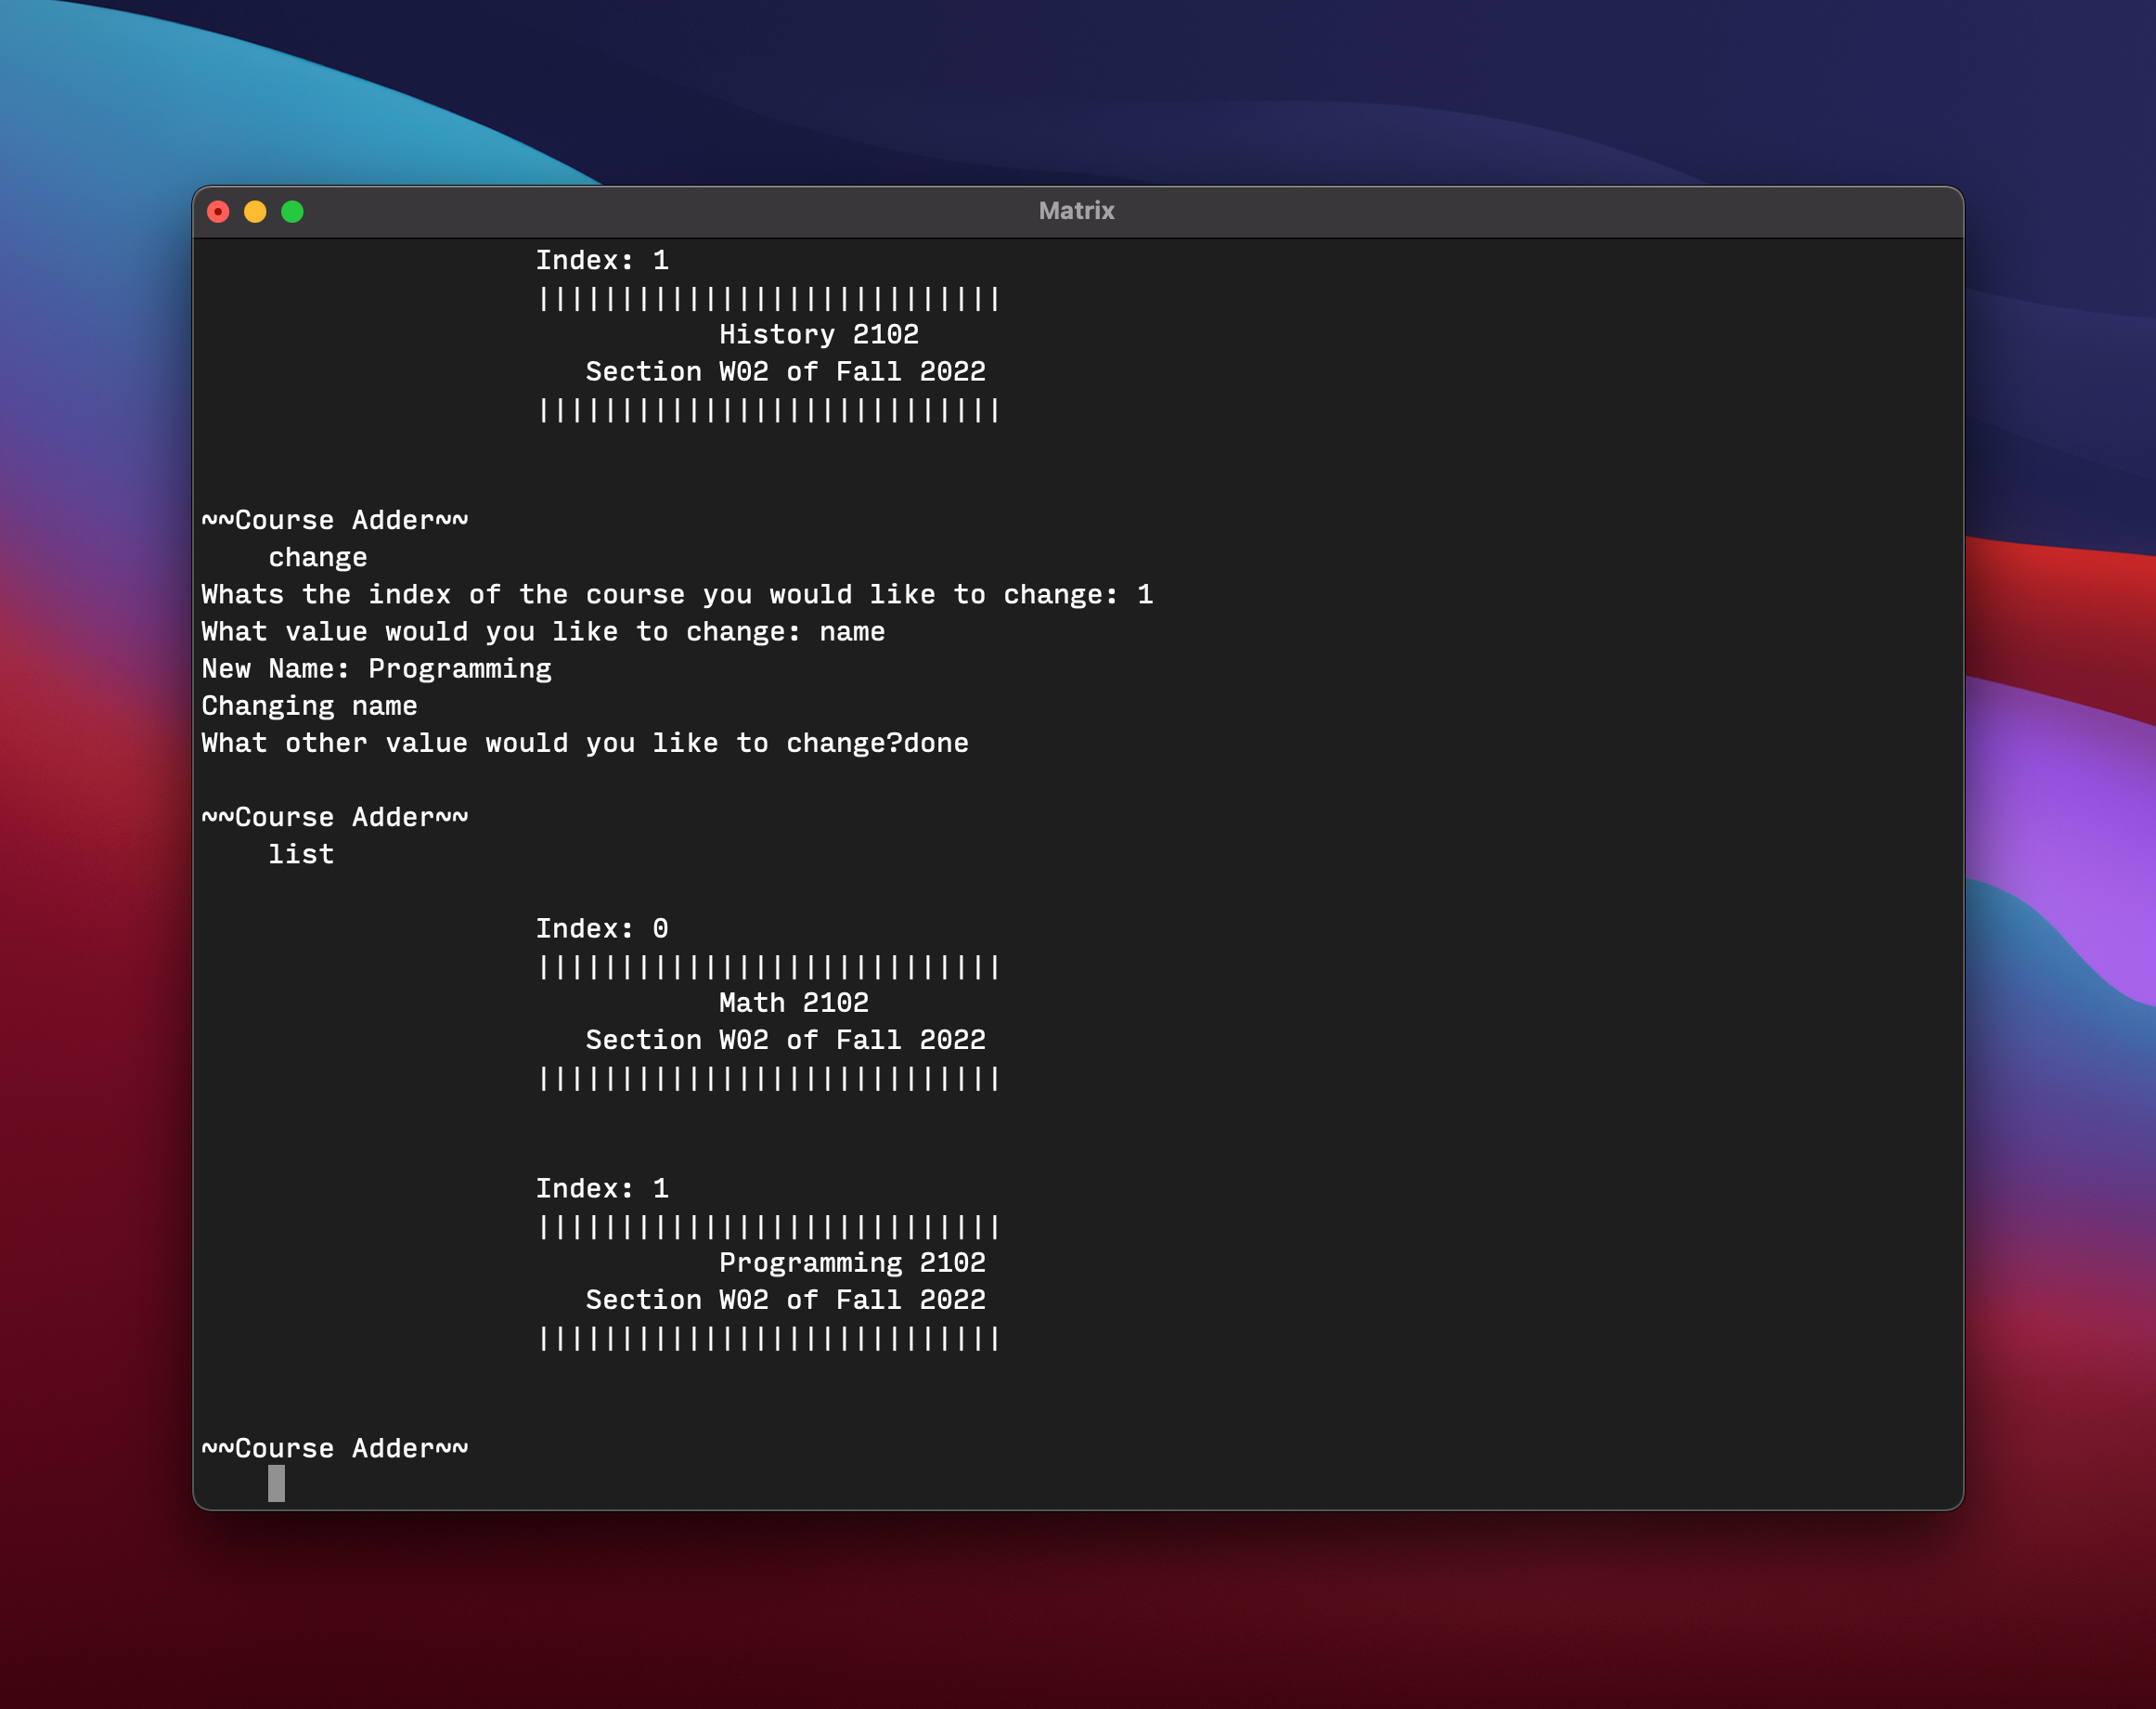
\includegraphics[width = \textwidth]{listchange}

\section{Summary}
After finishing this assignment I had a greater understanding of python than I did coming in. 
Python is rarely a language I use but with the tools learned in the class about how languages are formulated it made it seem easier to but the basic building blocks of language together and use them for my own ends such as in this programming assignment. 
\end{document}

